\documentclass[11pt,a4paper]{article}

% Packages
\usepackage[utf8]{inputenc}
\usepackage[T1]{fontenc}
\usepackage{amsmath,amssymb}
\usepackage{graphicx}
\usepackage{booktabs}
\usepackage{array}
\usepackage{tikz}
\usetikzlibrary{shapes,arrows,positioning,fit,calc,backgrounds,decorations.pathreplacing}
\usepackage{xcolor}
\usepackage[hidelinks]{hyperref}
\usepackage{geometry}
\geometry{margin=0.9in}
\usepackage{float}

% Colors
\definecolor{globalcolor}{RGB}{100, 149, 237}
\definecolor{statecolor}{RGB}{144, 238, 144}
\definecolor{actorcolor}{RGB}{255, 182, 108}
\definecolor{dynamicscolor}{RGB}{255, 160, 160}
\definecolor{temporalcolor}{RGB}{221, 160, 221}
\definecolor{fusioncolor}{RGB}{200, 200, 200}

\title{Cricket Ball Prediction Model:\\A Conceptual Guide}
\author{Architecture Documentation}
\date{\today}

\begin{document}

\maketitle

\begin{abstract}
This document provides a conceptual understanding of the CricketPredictor model. Rather than focusing on equations, we emphasize \textbf{what goes in}, \textbf{what comes out}, and \textbf{what each component intuitively represents}. The goal is to understand the model well enough to rewrite it.
\end{abstract}

\tableofcontents
\newpage

%==========================================
\section{The Big Picture}
%==========================================

\subsection{What the Model Does}

Given the current state of a cricket match, predict what happens on the next ball:

\begin{center}
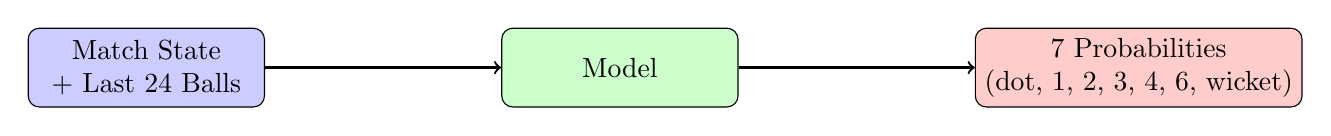
\begin{tikzpicture}[
    box/.style={rectangle, draw, rounded corners, minimum width=3cm, minimum height=1cm, align=center},
]
    \node[box, fill=blue!20] (input) {Match State\\+ Last 24 Balls};
    \node[box, fill=green!20, right=3cm of input] (model) {Model};
    \node[box, fill=red!20, right=3cm of model] (output) {7 Probabilities\\(dot, 1, 2, 3, 4, 6, wicket)};

    \draw[->, thick] (input) -- (model);
    \draw[->, thick] (model) -- (output);
\end{tikzpicture}
\end{center}

\subsection{Two Parallel Streams}

The model processes information through two parallel pathways that answer different questions:

\begin{figure}[H]
\centering
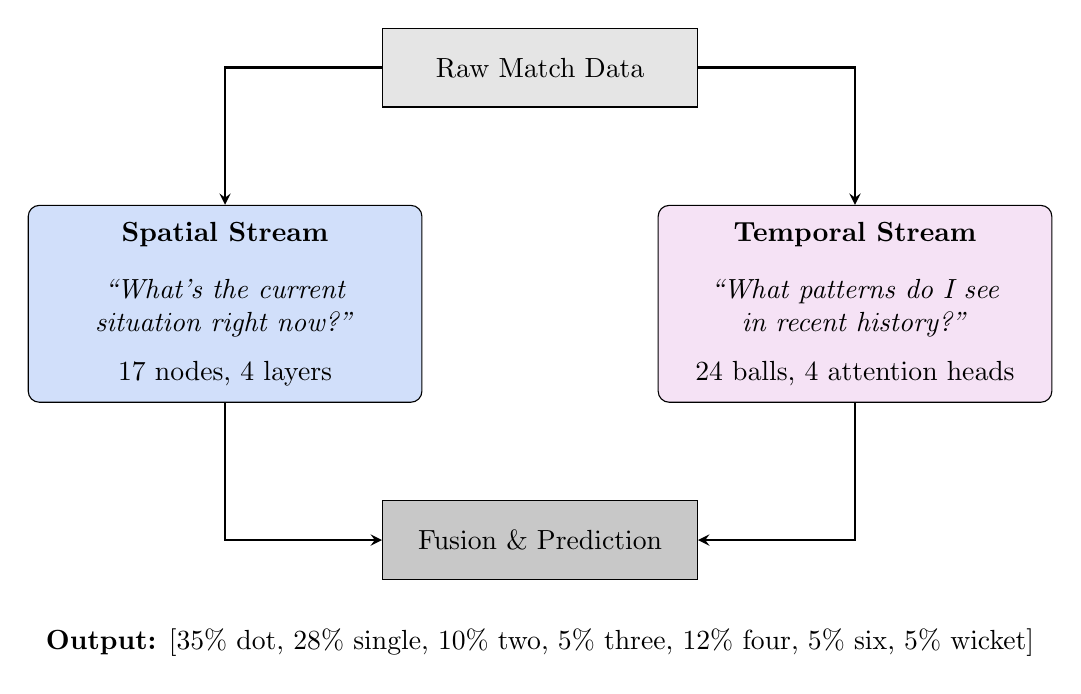
\begin{tikzpicture}[
    stream/.style={rectangle, draw, rounded corners, minimum width=5cm, minimum height=2.5cm, align=center},
    arrow/.style={->, thick, >=stealth}
]
    % Input
    \node[rectangle, draw, fill=gray!20, minimum width=4cm, minimum height=1cm] (input) at (0, 3) {Raw Match Data};

    % Two streams
    \node[stream, fill=globalcolor!30] (spatial) at (-4, 0) {
        \textbf{Spatial Stream}\\[0.3cm]
        \textit{``What's the current}\\
        \textit{situation right now?''}\\[0.2cm]
        17 nodes, 4 layers
    };

    \node[stream, fill=temporalcolor!30] (temporal) at (4, 0) {
        \textbf{Temporal Stream}\\[0.3cm]
        \textit{``What patterns do I see}\\
        \textit{in recent history?''}\\[0.2cm]
        24 balls, 4 attention heads
    };

    % Fusion
    \node[rectangle, draw, fill=fusioncolor, minimum width=4cm, minimum height=1cm] (fusion) at (0, -3) {Fusion \& Prediction};

    % Arrows
    \draw[arrow] (input) -| (spatial);
    \draw[arrow] (input) -| (temporal);
    \draw[arrow] (spatial) |- (fusion);
    \draw[arrow] (temporal) |- (fusion);

    % Output
    \node[below=0.5cm of fusion] (out) {\textbf{Output:} [35\% dot, 28\% single, 10\% two, 5\% three, 12\% four, 5\% six, 5\% wicket]};
\end{tikzpicture}
\caption{Dual-stream architecture: Spatial (current context) and Temporal (ball history)}
\end{figure}

%==========================================
\section{The Spatial Stream: HierarchicalGAT}
%==========================================

\subsection{The Core Idea}

Cricket has a natural hierarchy of factors that influence each ball:

\begin{figure}[H]
\centering
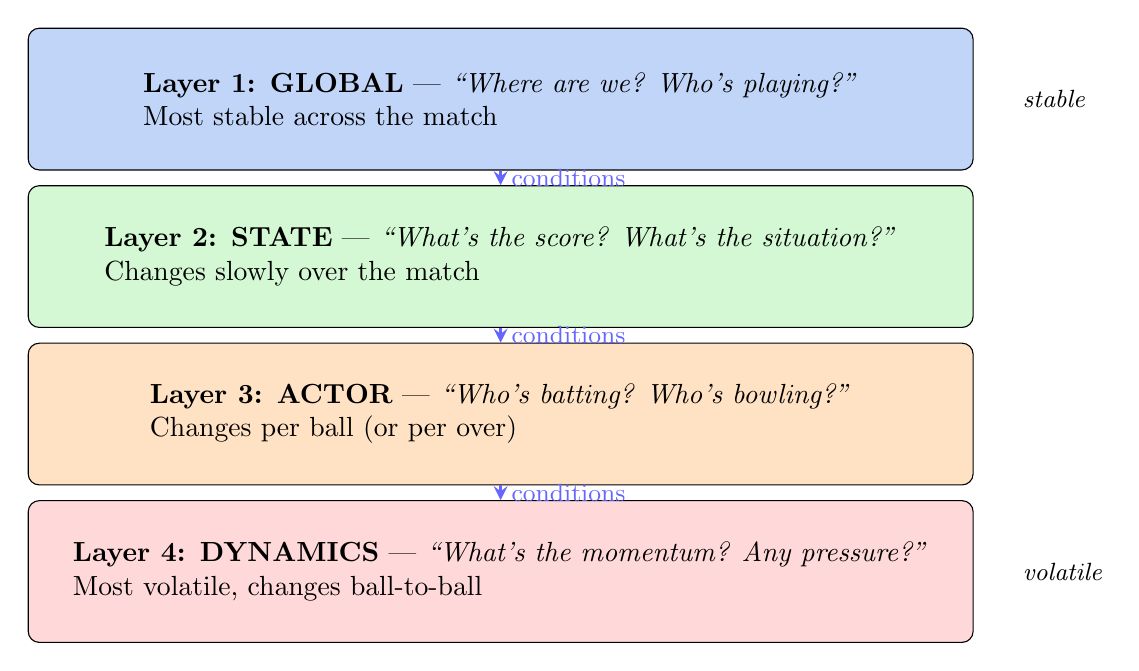
\begin{tikzpicture}[
    layer/.style={rectangle, draw, rounded corners, minimum width=12cm, minimum height=1.8cm, align=left},
    arrow/.style={->, thick, >=stealth}
]
    % Layers
    \node[layer, fill=globalcolor!40] (global) at (0, 6) {
        \textbf{Layer 1: GLOBAL} --- \textit{``Where are we? Who's playing?''}\\
        Most stable across the match
    };

    \node[layer, fill=statecolor!40] (state) at (0, 4) {
        \textbf{Layer 2: STATE} --- \textit{``What's the score? What's the situation?''}\\
        Changes slowly over the match
    };

    \node[layer, fill=actorcolor!40] (actor) at (0, 2) {
        \textbf{Layer 3: ACTOR} --- \textit{``Who's batting? Who's bowling?''}\\
        Changes per ball (or per over)
    };

    \node[layer, fill=dynamicscolor!40] (dynamics) at (0, 0) {
        \textbf{Layer 4: DYNAMICS} --- \textit{``What's the momentum? Any pressure?''}\\
        Most volatile, changes ball-to-ball
    };

    % Conditioning arrows
    \draw[arrow, very thick, blue!60] (global.south) -- node[right, font=\small] {conditions} (state.north);
    \draw[arrow, very thick, blue!60] (state.south) -- node[right, font=\small] {conditions} (actor.north);
    \draw[arrow, very thick, blue!60] (actor.south) -- node[right, font=\small] {conditions} (dynamics.north);

    % Side labels
    \node[right=0.5cm of global.east, font=\small\itshape] {stable};
    \node[right=0.5cm of dynamics.east, font=\small\itshape] {volatile};
\end{tikzpicture}
\caption{The hierarchical structure: higher layers condition lower layers}
\end{figure}

\subsection{Key Insight: Top-Down Conditioning}

Each layer receives context from the layer above it:
\begin{itemize}
    \item \textbf{State} knows about the venue and teams (global context)
    \item \textbf{Actor} knows about the match situation (state context)
    \item \textbf{Dynamics} knows about the current batter/bowler (actor context)
\end{itemize}

This mirrors how a cricket expert thinks: ``At the MCG (global), with India needing 50 off 30 (state), Rohit facing Bumrah (actor), after two dot balls (dynamics)...''

\newpage
\subsection{Layer 1: Global Context}

\begin{figure}[H]
\centering
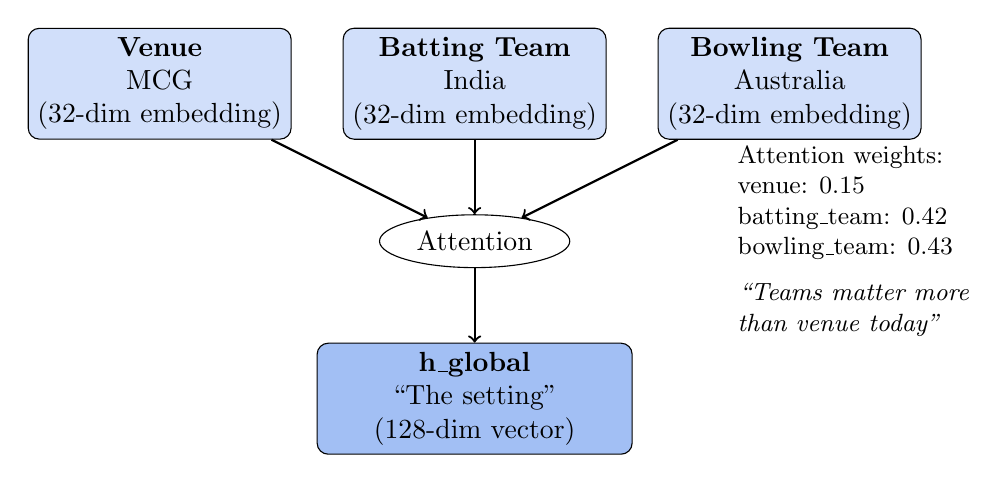
\begin{tikzpicture}[
    node/.style={rectangle, draw, rounded corners, minimum width=3cm, minimum height=1.2cm, align=center, fill=globalcolor!30},
    output/.style={rectangle, draw, rounded corners, minimum width=4cm, minimum height=1cm, align=center, fill=globalcolor!60},
]
    % Input nodes
    \node[node] (venue) at (-4, 0) {\textbf{Venue}\\MCG\\(32-dim embedding)};
    \node[node] (batteam) at (0, 0) {\textbf{Batting Team}\\India\\(32-dim embedding)};
    \node[node] (bowlteam) at (4, 0) {\textbf{Bowling Team}\\Australia\\(32-dim embedding)};

    % Attention
    \node[ellipse, draw, fill=white, minimum width=2cm] (attn) at (0, -2) {Attention};

    % Output
    \node[output] (output) at (0, -4) {\textbf{h\_global}\\``The setting''\\(128-dim vector)};

    % Arrows
    \draw[->, thick] (venue) -- (attn);
    \draw[->, thick] (batteam) -- (attn);
    \draw[->, thick] (bowlteam) -- (attn);
    \draw[->, thick] (attn) -- (output);

    % Attention weights
    \node[right=2cm of attn, align=left, font=\small] {
        Attention weights:\\
        venue: 0.15\\
        batting\_team: 0.42\\
        bowling\_team: 0.43\\[0.2cm]
        \textit{``Teams matter more}\\
        \textit{than venue today''}
    };
\end{tikzpicture}
\caption{Layer 1: Global context aggregation}
\end{figure}

\textbf{Inputs:}
\begin{itemize}
    \item \texttt{venue}: 32-dim learned embedding (encodes pitch type, ground size, typical scores)
    \item \texttt{batting\_team}: 32-dim learned embedding (encodes team's batting style)
    \item \texttt{bowling\_team}: 32-dim learned embedding (encodes team's bowling attack)
\end{itemize}

\textbf{Output:} \texttt{h\_global} (128-dim) --- represents ``the setting'' for this match.

\textbf{Intuition:} A learned query asks ``What combination of venue and teams matters for this prediction?'' and produces a weighted summary.

\newpage
\subsection{Layer 2: Match State}

\begin{figure}[H]
\centering
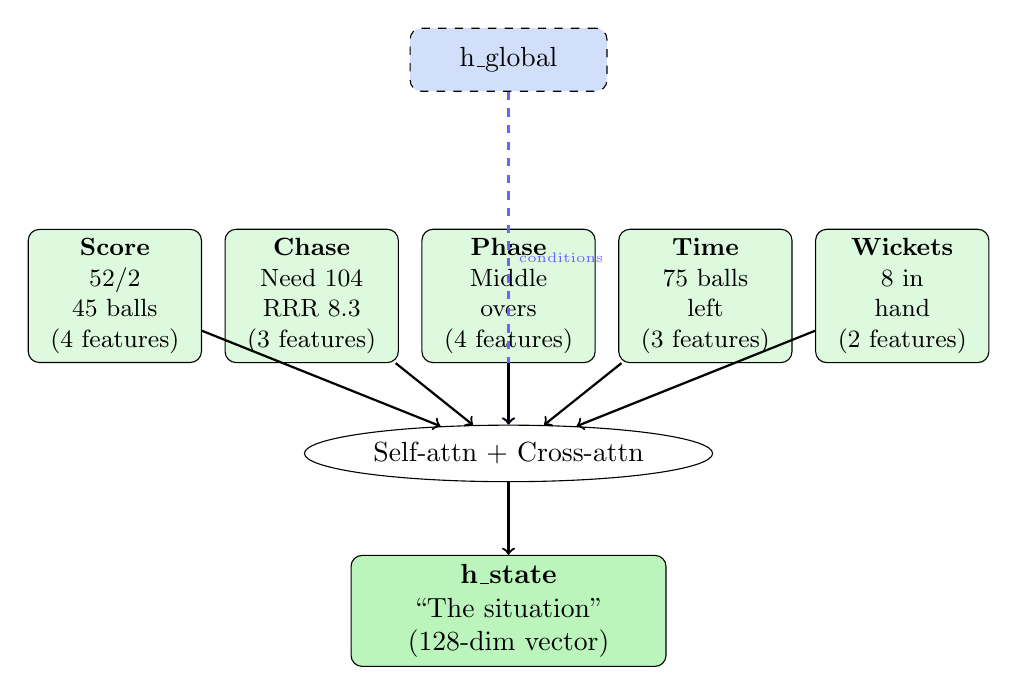
\begin{tikzpicture}[
    node/.style={rectangle, draw, rounded corners, minimum width=2.2cm, minimum height=1.5cm, align=center, fill=statecolor!30, font=\small},
    output/.style={rectangle, draw, rounded corners, minimum width=4cm, minimum height=1cm, align=center, fill=statecolor!60},
    context/.style={rectangle, draw, dashed, rounded corners, minimum width=2.5cm, minimum height=0.8cm, align=center, fill=globalcolor!30},
]
    % Context from above
    \node[context] (global) at (0, 3) {h\_global};

    % Input nodes
    \node[node] (score) at (-5, 0) {\textbf{Score}\\52/2\\45 balls\\(4 features)};
    \node[node] (chase) at (-2.5, 0) {\textbf{Chase}\\Need 104\\RRR 8.3\\(3 features)};
    \node[node] (phase) at (0, 0) {\textbf{Phase}\\Middle\\overs\\(4 features)};
    \node[node] (time) at (2.5, 0) {\textbf{Time}\\75 balls\\left\\(3 features)};
    \node[node] (wicket) at (5, 0) {\textbf{Wickets}\\8 in\\hand\\(2 features)};

    % Processing
    \node[ellipse, draw, fill=white, minimum width=3cm] (proc) at (0, -2) {Self-attn + Cross-attn};

    % Output
    \node[output] (output) at (0, -4) {\textbf{h\_state}\\``The situation''\\(128-dim vector)};

    % Arrows
    \draw[->, thick, dashed, blue!60] (global) -- node[right, font=\tiny] {conditions} (proc);
    \foreach \n in {score, chase, phase, time, wicket} {
        \draw[->, thick] (\n) -- (proc);
    }
    \draw[->, thick] (proc) -- (output);
\end{tikzpicture}
\caption{Layer 2: Match state with conditioning from global}
\end{figure}

\textbf{Inputs (5 nodes, 16 features total):}

\begin{table}[H]
\centering
\begin{tabular}{lll}
\toprule
Node & Raw Features & Intuition \\
\midrule
\texttt{score\_state} & score/200, wickets/10, balls/120, innings & Current score status \\
\texttt{chase\_state} & runs\_needed/200, RRR/15, is\_chase & Chase equation \\
\texttt{phase\_state} & powerplay, middle, death, progress & Match phase \\
\texttt{time\_pressure} & balls\_left/120, urgency, is\_death & Time remaining \\
\texttt{wicket\_buffer} & wickets\_in\_hand/10, is\_danger & Wicket cushion \\
\bottomrule
\end{tabular}
\end{table}

\textbf{Processing:}
\begin{enumerate}
    \item Self-attention: State nodes inform each other (e.g., chase relates to score)
    \item Cross-attention: Nodes attend to h\_global (situation interpreted through venue/teams)
    \item Pool: Compress 5 nodes into one vector
\end{enumerate}

\textbf{Output:} \texttt{h\_state} (128-dim) --- represents ``the match situation.''

\newpage
\subsection{Layer 3: Actor (The Matchup)}

\begin{figure}[H]
\centering
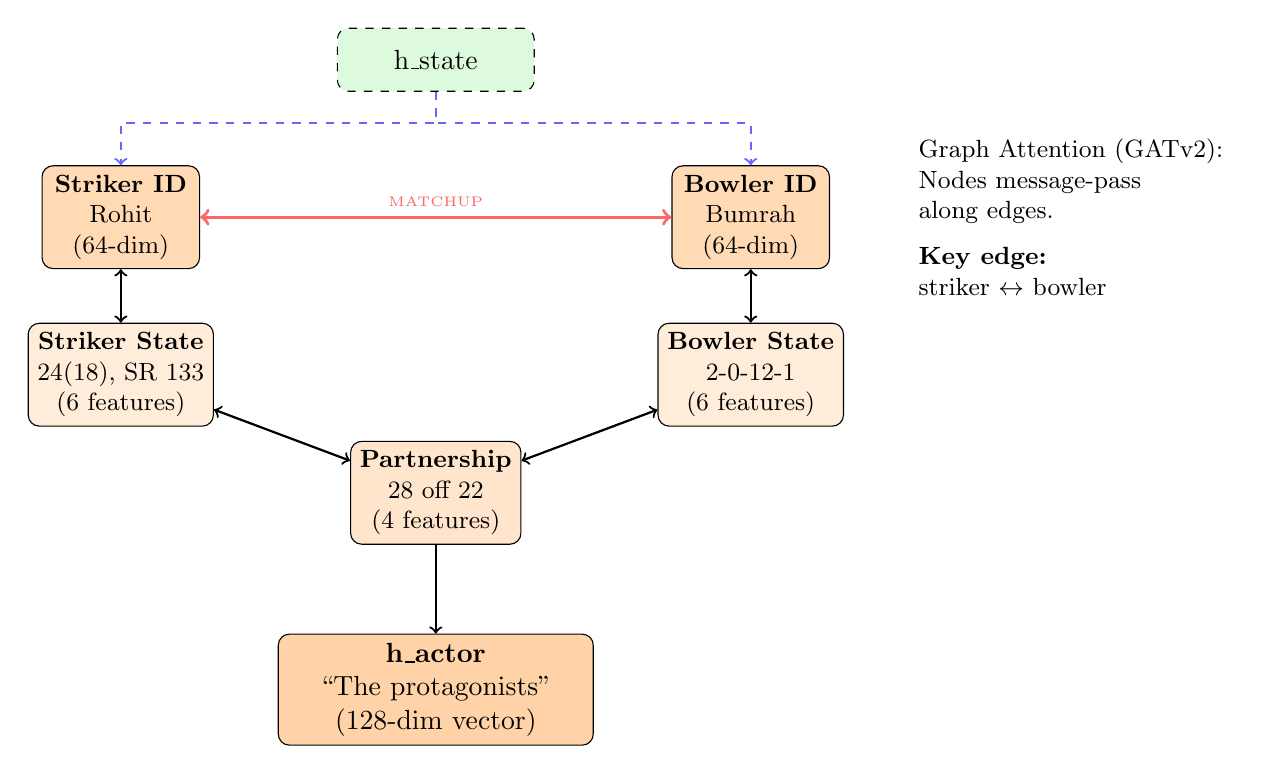
\begin{tikzpicture}[
    node/.style={rectangle, draw, rounded corners, minimum width=2cm, minimum height=1.2cm, align=center, font=\small},
    identity/.style={node, fill=actorcolor!50},
    state/.style={node, fill=actorcolor!25},
    partnership/.style={node, fill=actorcolor!35},
    output/.style={rectangle, draw, rounded corners, minimum width=4cm, minimum height=1cm, align=center, fill=actorcolor!60},
    context/.style={rectangle, draw, dashed, rounded corners, minimum width=2.5cm, minimum height=0.8cm, align=center, fill=statecolor!30},
]
    % Context from above
    \node[context] (state) at (0, 4) {h\_state};

    % Striker side
    \node[identity] (striker_id) at (-4, 2) {\textbf{Striker ID}\\Rohit\\(64-dim)};
    \node[state] (striker_st) at (-4, 0) {\textbf{Striker State}\\24(18), SR 133\\(6 features)};

    % Bowler side
    \node[identity] (bowler_id) at (4, 2) {\textbf{Bowler ID}\\Bumrah\\(64-dim)};
    \node[state] (bowler_st) at (4, 0) {\textbf{Bowler State}\\2-0-12-1\\(6 features)};

    % Partnership
    \node[partnership] (partner) at (0, -1.5) {\textbf{Partnership}\\28 off 22\\(4 features)};

    % Graph edges
    \draw[<->, very thick, red!60] (striker_id) -- node[above, font=\tiny] {MATCHUP} (bowler_id);
    \draw[<->, thick] (striker_id) -- (striker_st);
    \draw[<->, thick] (bowler_id) -- (bowler_st);
    \draw[<->, thick] (striker_st) -- (partner);
    \draw[<->, thick] (bowler_st) -- (partner);

    % Conditioning
    \draw[->, thick, dashed, blue!60] (state) -- ++(0,-0.8) -| (striker_id);
    \draw[->, thick, dashed, blue!60] (state) -- ++(0,-0.8) -| (bowler_id);

    % Output
    \node[output] (output) at (0, -4) {\textbf{h\_actor}\\``The protagonists''\\(128-dim vector)};

    \draw[->, thick] (partner) -- (output);

    % Note
    \node[right=1cm of bowler_id, align=left, font=\small] {
        Graph Attention (GATv2):\\
        Nodes message-pass\\
        along edges.\\[0.2cm]
        \textbf{Key edge:}\\
        striker $\leftrightarrow$ bowler
    };
\end{tikzpicture}
\caption{Layer 3: Actor graph with fixed edge structure}
\end{figure}

\textbf{Inputs (5 nodes):}

\begin{table}[H]
\centering
\begin{tabular}{lll}
\toprule
Node & What It Contains & Dimension \\
\midrule
\texttt{striker\_identity} & WHO is batting (learned embedding) & 64 \\
\texttt{striker\_state} & HOW they're doing today (runs, balls, SR, dots, setness, boundaries) & 6 \\
\texttt{bowler\_identity} & WHO is bowling (learned embedding) & 64 \\
\texttt{bowler\_state} & HOW they're doing today (balls, runs, wickets, econ, dots, threat) & 6 \\
\texttt{partnership} & Current partnership stats (runs, balls, RR, stability) & 4 \\
\bottomrule
\end{tabular}
\end{table}

\textbf{The Graph Structure:}
\begin{itemize}
    \item Striker ID $\leftrightarrow$ Striker State (who I am $\leftrightarrow$ how I'm playing)
    \item Bowler ID $\leftrightarrow$ Bowler State (same for bowler)
    \item \textbf{Striker ID $\leftrightarrow$ Bowler ID} (THE MATCHUP --- the key edge!)
    \item States $\leftrightarrow$ Partnership (performance affects partnership)
\end{itemize}

\textbf{Output:} \texttt{h\_actor} (128-dim) --- represents ``the current protagonists and their duel.''

\newpage
\subsection{Layer 4: Dynamics}

\begin{figure}[H]
\centering
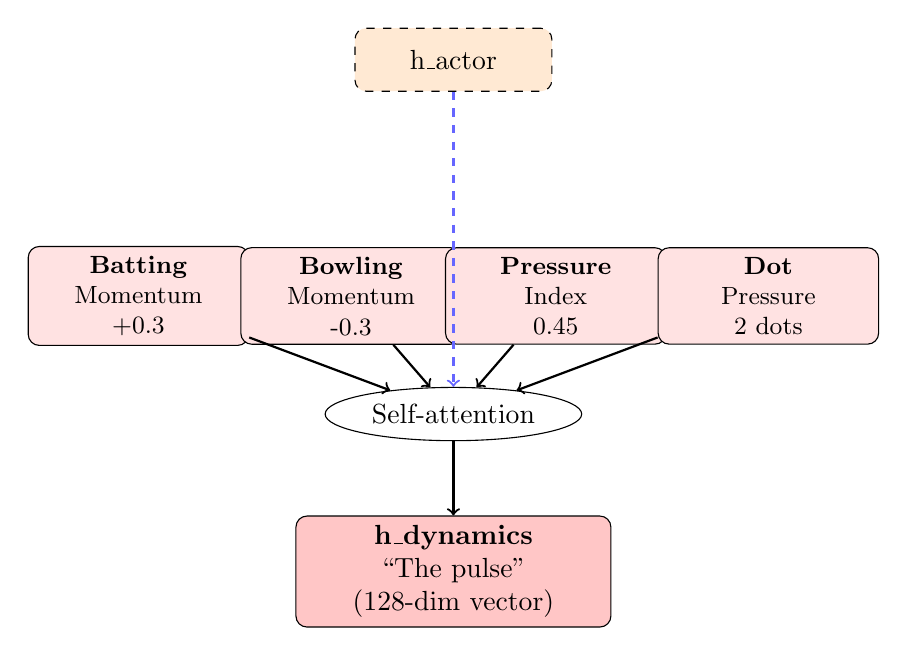
\begin{tikzpicture}[
    node/.style={rectangle, draw, rounded corners, minimum width=2.8cm, minimum height=1.2cm, align=center, fill=dynamicscolor!30, font=\small},
    output/.style={rectangle, draw, rounded corners, minimum width=4cm, minimum height=1cm, align=center, fill=dynamicscolor!60},
    context/.style={rectangle, draw, dashed, rounded corners, minimum width=2.5cm, minimum height=0.8cm, align=center, fill=actorcolor!30},
]
    % Context from above
    \node[context] (actor) at (0, 3) {h\_actor};

    % Input nodes
    \node[node] (batmom) at (-4, 0) {\textbf{Batting}\\Momentum\\+0.3};
    \node[node] (bowlmom) at (-1.3, 0) {\textbf{Bowling}\\Momentum\\-0.3};
    \node[node] (pressure) at (1.3, 0) {\textbf{Pressure}\\Index\\0.45};
    \node[node] (dots) at (4, 0) {\textbf{Dot}\\Pressure\\2 dots};

    % Processing
    \node[ellipse, draw, fill=white] (attn) at (0, -1.5) {Self-attention};

    % Output
    \node[output] (output) at (0, -3.5) {\textbf{h\_dynamics}\\``The pulse''\\(128-dim vector)};

    % Arrows
    \draw[->, thick, dashed, blue!60] (actor) -- (attn);
    \foreach \n in {batmom, bowlmom, pressure, dots} {
        \draw[->, thick] (\n) -- (attn);
    }
    \draw[->, thick] (attn) -- (output);
\end{tikzpicture}
\caption{Layer 4: Dynamics --- the most volatile layer}
\end{figure}

\textbf{Inputs (4 nodes, 5 features total):}

\begin{table}[H]
\centering
\begin{tabular}{lll}
\toprule
Node & Raw Value & Intuition \\
\midrule
\texttt{batting\_momentum} & (recent\_RR / expected\_RR) - 1 & Are they scoring freely? \\
\texttt{bowling\_momentum} & Negative of batting & Is the bowler on top? \\
\texttt{pressure\_index} & Composite of wickets + RRR + stage & Overall pressure level \\
\texttt{dot\_pressure} & consecutive\_dots, balls\_since\_boundary & Building pressure \\
\bottomrule
\end{tabular}
\end{table}

\textbf{Output:} \texttt{h\_dynamics} (128-dim) --- represents ``the current momentum and pressure.''

\newpage
\subsection{Combining the Four Layers}

\begin{figure}[H]
\centering
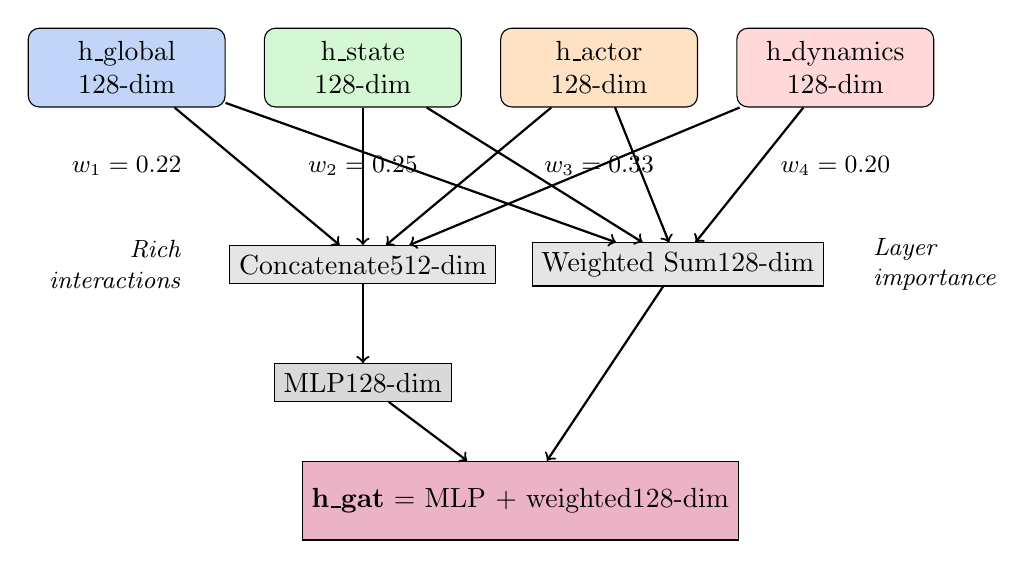
\begin{tikzpicture}[
    layer/.style={rectangle, draw, rounded corners, minimum width=2.5cm, minimum height=1cm, align=center},
    arrow/.style={->, thick}
]
    % Four layer outputs
    \node[layer, fill=globalcolor!40] (g) at (-4.5, 0) {h\_global\\128-dim};
    \node[layer, fill=statecolor!40] (s) at (-1.5, 0) {h\_state\\128-dim};
    \node[layer, fill=actorcolor!40] (a) at (1.5, 0) {h\_actor\\128-dim};
    \node[layer, fill=dynamicscolor!40] (d) at (4.5, 0) {h\_dynamics\\128-dim};

    % Learned weights
    \node[below=0.5cm of g, font=\small] {$w_1 = 0.22$};
    \node[below=0.5cm of s, font=\small] {$w_2 = 0.25$};
    \node[below=0.5cm of a, font=\small] {$w_3 = 0.33$};
    \node[below=0.5cm of d, font=\small] {$w_4 = 0.20$};

    % Two fusion paths
    \node[rectangle, draw, fill=gray!20, minimum width=3cm] (concat) at (-1.5, -2.5) {Concatenate\\512-dim};
    \node[rectangle, draw, fill=gray!20, minimum width=3cm] (weighted) at (2.5, -2.5) {Weighted Sum\\128-dim};

    % MLP
    \node[rectangle, draw, fill=gray!30, minimum width=2cm] (mlp) at (-1.5, -4) {MLP\\128-dim};

    % Final
    \node[rectangle, draw, fill=purple!30, minimum width=4cm, minimum height=1cm] (out) at (0.5, -5.5) {\textbf{h\_gat} = MLP + weighted\\128-dim};

    % Arrows
    \draw[arrow] (g) -- (concat);
    \draw[arrow] (s) -- (concat);
    \draw[arrow] (a) -- (concat);
    \draw[arrow] (d) -- (concat);

    \draw[arrow] (g) -- (weighted);
    \draw[arrow] (s) -- (weighted);
    \draw[arrow] (a) -- (weighted);
    \draw[arrow] (d) -- (weighted);

    \draw[arrow] (concat) -- (mlp);
    \draw[arrow] (mlp) -- (out);
    \draw[arrow] (weighted) -- (out);

    % Labels
    \node[left=0.5cm of concat, font=\small\itshape, align=right] {Rich\\interactions};
    \node[right=0.5cm of weighted, font=\small\itshape, align=left] {Layer\\importance};
\end{tikzpicture}
\caption{Fusion: both concatenation (for interactions) and weighted sum (for importance)}
\end{figure}

\textbf{Why two fusion methods?}
\begin{itemize}
    \item \textbf{Weighted sum}: Learns which layer matters most (interpretable --- ``actor layer drives this prediction'')
    \item \textbf{Concatenation + MLP}: Learns interactions between layers (``venue + actor combination matters'')
\end{itemize}

\textbf{Output:} \texttt{h\_gat} (128-dim) --- the complete spatial representation.

%==========================================
\newpage
\section{The Temporal Stream}
%==========================================

\subsection{The Core Idea}

While the spatial stream asks ``What's the situation NOW?'', the temporal stream asks ``What patterns do I see in RECENT HISTORY?''

\begin{figure}[H]
\centering
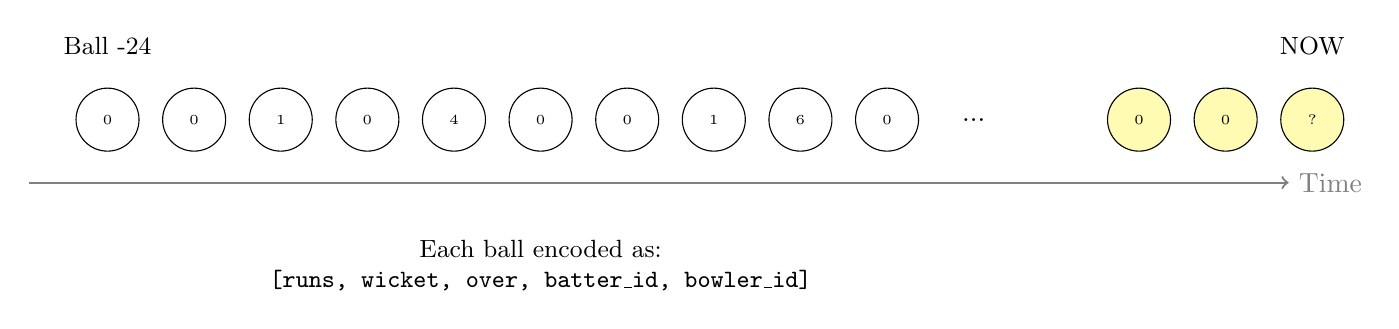
\begin{tikzpicture}[
    ball/.style={circle, draw, minimum size=0.8cm, font=\tiny},
    arrow/.style={->, thick}
]
    % Ball sequence
    \foreach \i/\r in {0/0, 1/0, 2/1, 3/0, 4/4, 5/0, 6/0, 7/1, 8/6, 9/0} {
        \node[ball, fill=white] (b\i) at (\i*1.1, 0) {\r};
    }
    \node at (11, 0) {...};
    \foreach \i/\r in {21/0, 22/0, 23/?} {
        \node[ball, fill=yellow!30] (b\i) at (\i*1.1 - 10, 0) {\r};
    }

    % Labels
    \node[above=0.3cm of b0, font=\small] {Ball -24};
    \node[above=0.3cm of b23, font=\small] {NOW};

    % Arrow showing time
    \draw[arrow, gray] (-1, -0.8) -- (15, -0.8) node[right] {Time};

    % Annotation
    \node[below=1cm of b5, align=center, font=\small] {
        Each ball encoded as:\\
        \texttt{[runs, wicket, over, batter\_id, bowler\_id]}
    };
\end{tikzpicture}
\caption{The temporal input: last 24 balls of history}
\end{figure}

\subsection{Ball Embedding}

Each historical ball is converted to a 128-dim vector:

\begin{figure}[H]
\centering
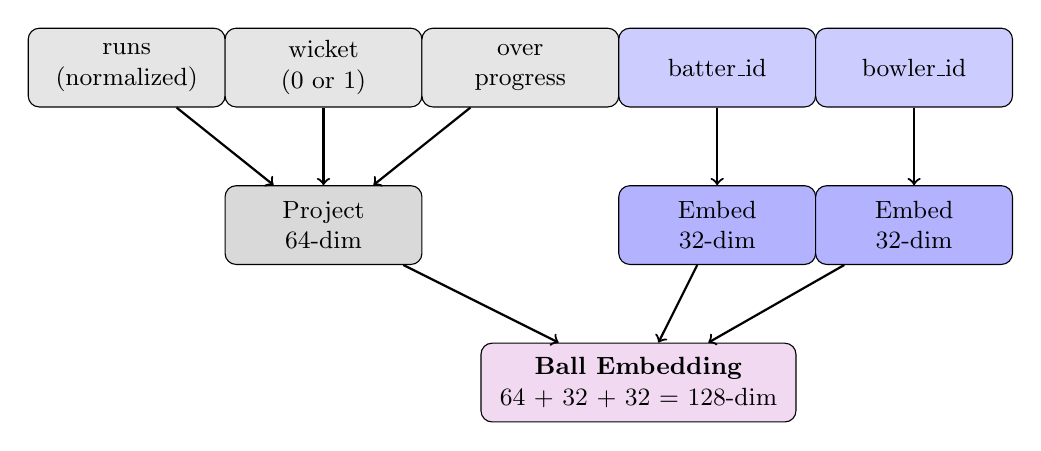
\begin{tikzpicture}[
    box/.style={rectangle, draw, rounded corners, minimum width=2.5cm, minimum height=1cm, align=center, font=\small},
]
    % Inputs
    \node[box, fill=gray!20] (runs) at (-4, 2) {runs\\(normalized)};
    \node[box, fill=gray!20] (wicket) at (-1.5, 2) {wicket\\(0 or 1)};
    \node[box, fill=gray!20] (over) at (1, 2) {over\\progress};
    \node[box, fill=blue!20] (batter) at (3.5, 2) {batter\_id};
    \node[box, fill=blue!20] (bowler) at (6, 2) {bowler\_id};

    % Processing
    \node[box, fill=gray!30] (proj) at (-1.5, 0) {Project\\64-dim};
    \node[box, fill=blue!30] (embed1) at (3.5, 0) {Embed\\32-dim};
    \node[box, fill=blue!30] (embed2) at (6, 0) {Embed\\32-dim};

    % Concat
    \node[box, fill=temporalcolor!40, minimum width=4cm] (concat) at (2.5, -2) {\textbf{Ball Embedding}\\64 + 32 + 32 = 128-dim};

    % Arrows
    \draw[->, thick] (runs) -- (proj);
    \draw[->, thick] (wicket) -- (proj);
    \draw[->, thick] (over) -- (proj);
    \draw[->, thick] (batter) -- (embed1);
    \draw[->, thick] (bowler) -- (embed2);

    \draw[->, thick] (proj) -- (concat);
    \draw[->, thick] (embed1) -- (concat);
    \draw[->, thick] (embed2) -- (concat);
\end{tikzpicture}
\caption{How each ball becomes a 128-dim embedding}
\end{figure}

\subsection{Specialized Attention Heads}

The key innovation: \textbf{4 attention heads with different biases}:

\begin{figure}[H]
\centering
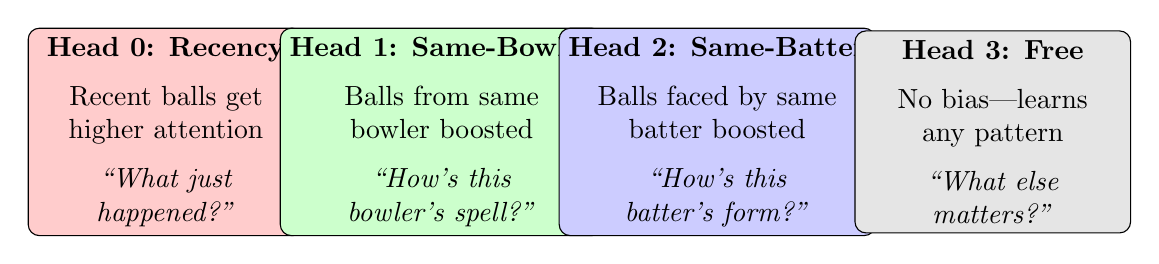
\begin{tikzpicture}[
    head/.style={rectangle, draw, rounded corners, minimum width=3.5cm, minimum height=2.5cm, align=center},
]
    \node[head, fill=red!20] (h0) at (-5, 0) {
        \textbf{Head 0: Recency}\\[0.2cm]
        Recent balls get\\
        higher attention\\[0.2cm]
        \textit{``What just}\\
        \textit{happened?''}
    };

    \node[head, fill=green!20] (h1) at (-1.5, 0) {
        \textbf{Head 1: Same-Bowler}\\[0.2cm]
        Balls from same\\
        bowler boosted\\[0.2cm]
        \textit{``How's this}\\
        \textit{bowler's spell?''}
    };

    \node[head, fill=blue!20] (h2) at (2, 0) {
        \textbf{Head 2: Same-Batter}\\[0.2cm]
        Balls faced by same\\
        batter boosted\\[0.2cm]
        \textit{``How's this}\\
        \textit{batter's form?''}
    };

    \node[head, fill=gray!20] (h3) at (5.5, 0) {
        \textbf{Head 3: Free}\\[0.2cm]
        No bias---learns\\
        any pattern\\[0.2cm]
        \textit{``What else}\\
        \textit{matters?''}
    };
\end{tikzpicture}
\caption{Four specialized attention heads encode cricket intuition}
\end{figure}

\textbf{How the biases work:}
\begin{itemize}
    \item \textbf{Recency}: Adds $\alpha \cdot \frac{\text{position}}{24}$ to attention scores (ball 24 gets +$\alpha$, ball 1 gets ~0)
    \item \textbf{Same-Bowler}: Adds $\beta$ to attention when bowler matches (e.g., all Bumrah balls get +$\beta$)
    \item \textbf{Same-Batter}: Adds $\gamma$ to attention when batter matches
    \item $\alpha, \beta, \gamma$ are \textbf{learned} during training
\end{itemize}

\subsection{Query Token for Pooling}

After the transformer layers, we need to compress 24 balls into one vector:

\begin{figure}[H]
\centering
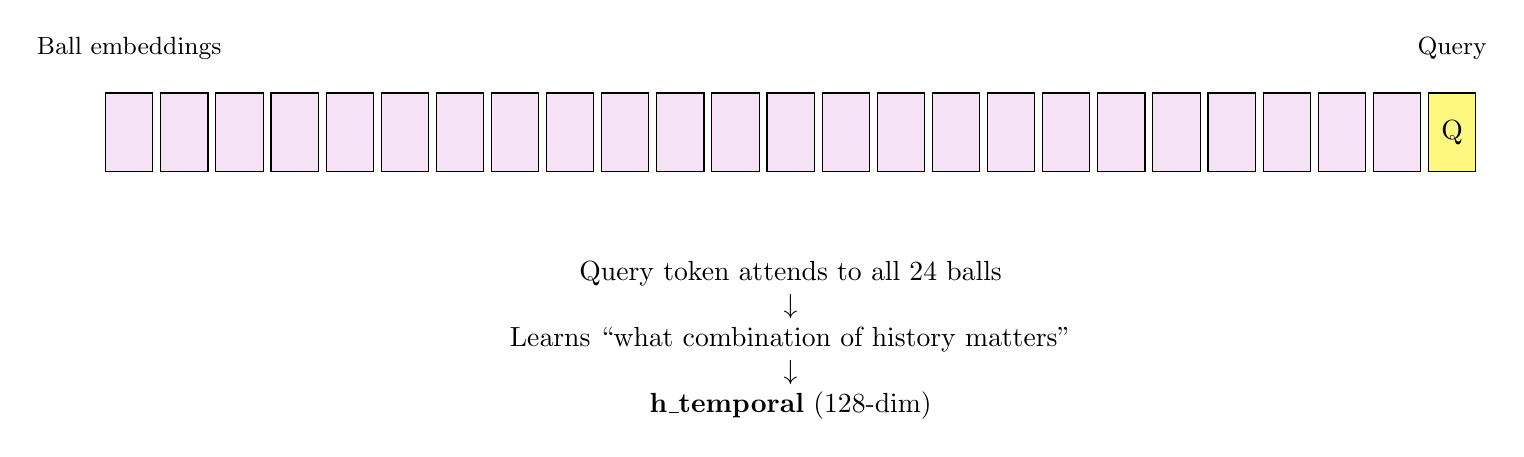
\begin{tikzpicture}[
    ball/.style={rectangle, draw, minimum width=0.6cm, minimum height=1cm, fill=temporalcolor!30},
    query/.style={rectangle, draw, minimum width=0.6cm, minimum height=1cm, fill=yellow!50},
]
    % Balls
    \foreach \i in {0,...,23} {
        \node[ball] (b\i) at (\i*0.7, 0) {};
    }
    \node[query] (q) at (24*0.7, 0) {Q};

    % Labels
    \node[above=0.3cm of b0, font=\small] {Ball embeddings};
    \node[above=0.3cm of q, font=\small] {Query};

    % Arrow
    \node[below=1cm of b12, align=center] {
        Query token attends to all 24 balls\\
        $\downarrow$\\
        Learns ``what combination of history matters''\\
        $\downarrow$\\
        \textbf{h\_temporal} (128-dim)
    };
\end{tikzpicture}
\caption{Learned query token pools the sequence}
\end{figure}

\textbf{Output:} \texttt{h\_temporal} (128-dim) --- the complete temporal representation.

%==========================================
\newpage
\section{Final Fusion and Prediction}
%==========================================

\begin{figure}[H]
\centering
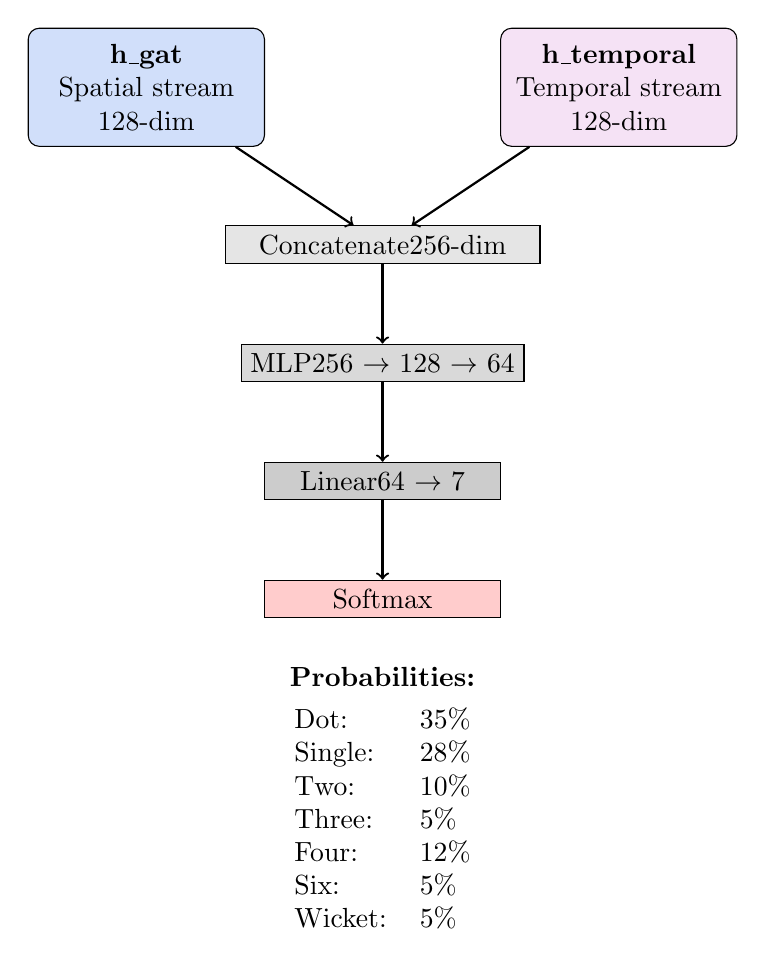
\begin{tikzpicture}[
    stream/.style={rectangle, draw, rounded corners, minimum width=3cm, minimum height=1.5cm, align=center},
    arrow/.style={->, thick}
]
    % Two streams
    \node[stream, fill=globalcolor!30] (spatial) at (-3, 3) {\textbf{h\_gat}\\Spatial stream\\128-dim};
    \node[stream, fill=temporalcolor!30] (temporal) at (3, 3) {\textbf{h\_temporal}\\Temporal stream\\128-dim};

    % Concat
    \node[rectangle, draw, fill=gray!20, minimum width=4cm] (concat) at (0, 1) {Concatenate\\256-dim};

    % MLP
    \node[rectangle, draw, fill=gray!30, minimum width=3cm] (mlp) at (0, -0.5) {MLP\\256 $\to$ 128 $\to$ 64};

    % Output layer
    \node[rectangle, draw, fill=gray!40, minimum width=3cm] (out) at (0, -2) {Linear\\64 $\to$ 7};

    % Softmax
    \node[rectangle, draw, fill=red!20, minimum width=3cm] (softmax) at (0, -3.5) {Softmax};

    % Final output
    \node[below=0.5cm of softmax, align=center] {
        \textbf{Probabilities:}\\[0.2cm]
        \begin{tabular}{ll}
        Dot: & 35\% \\
        Single: & 28\% \\
        Two: & 10\% \\
        Three: & 5\% \\
        Four: & 12\% \\
        Six: & 5\% \\
        Wicket: & 5\% \\
        \end{tabular}
    };

    % Arrows
    \draw[arrow] (spatial) -- (concat);
    \draw[arrow] (temporal) -- (concat);
    \draw[arrow] (concat) -- (mlp);
    \draw[arrow] (mlp) -- (out);
    \draw[arrow] (out) -- (softmax);
\end{tikzpicture}
\caption{Final fusion: combine spatial and temporal, predict 7 outcomes}
\end{figure}

%==========================================
\newpage
\section{Complete Data Flow Summary}
%==========================================

\begin{figure}[H]
\centering
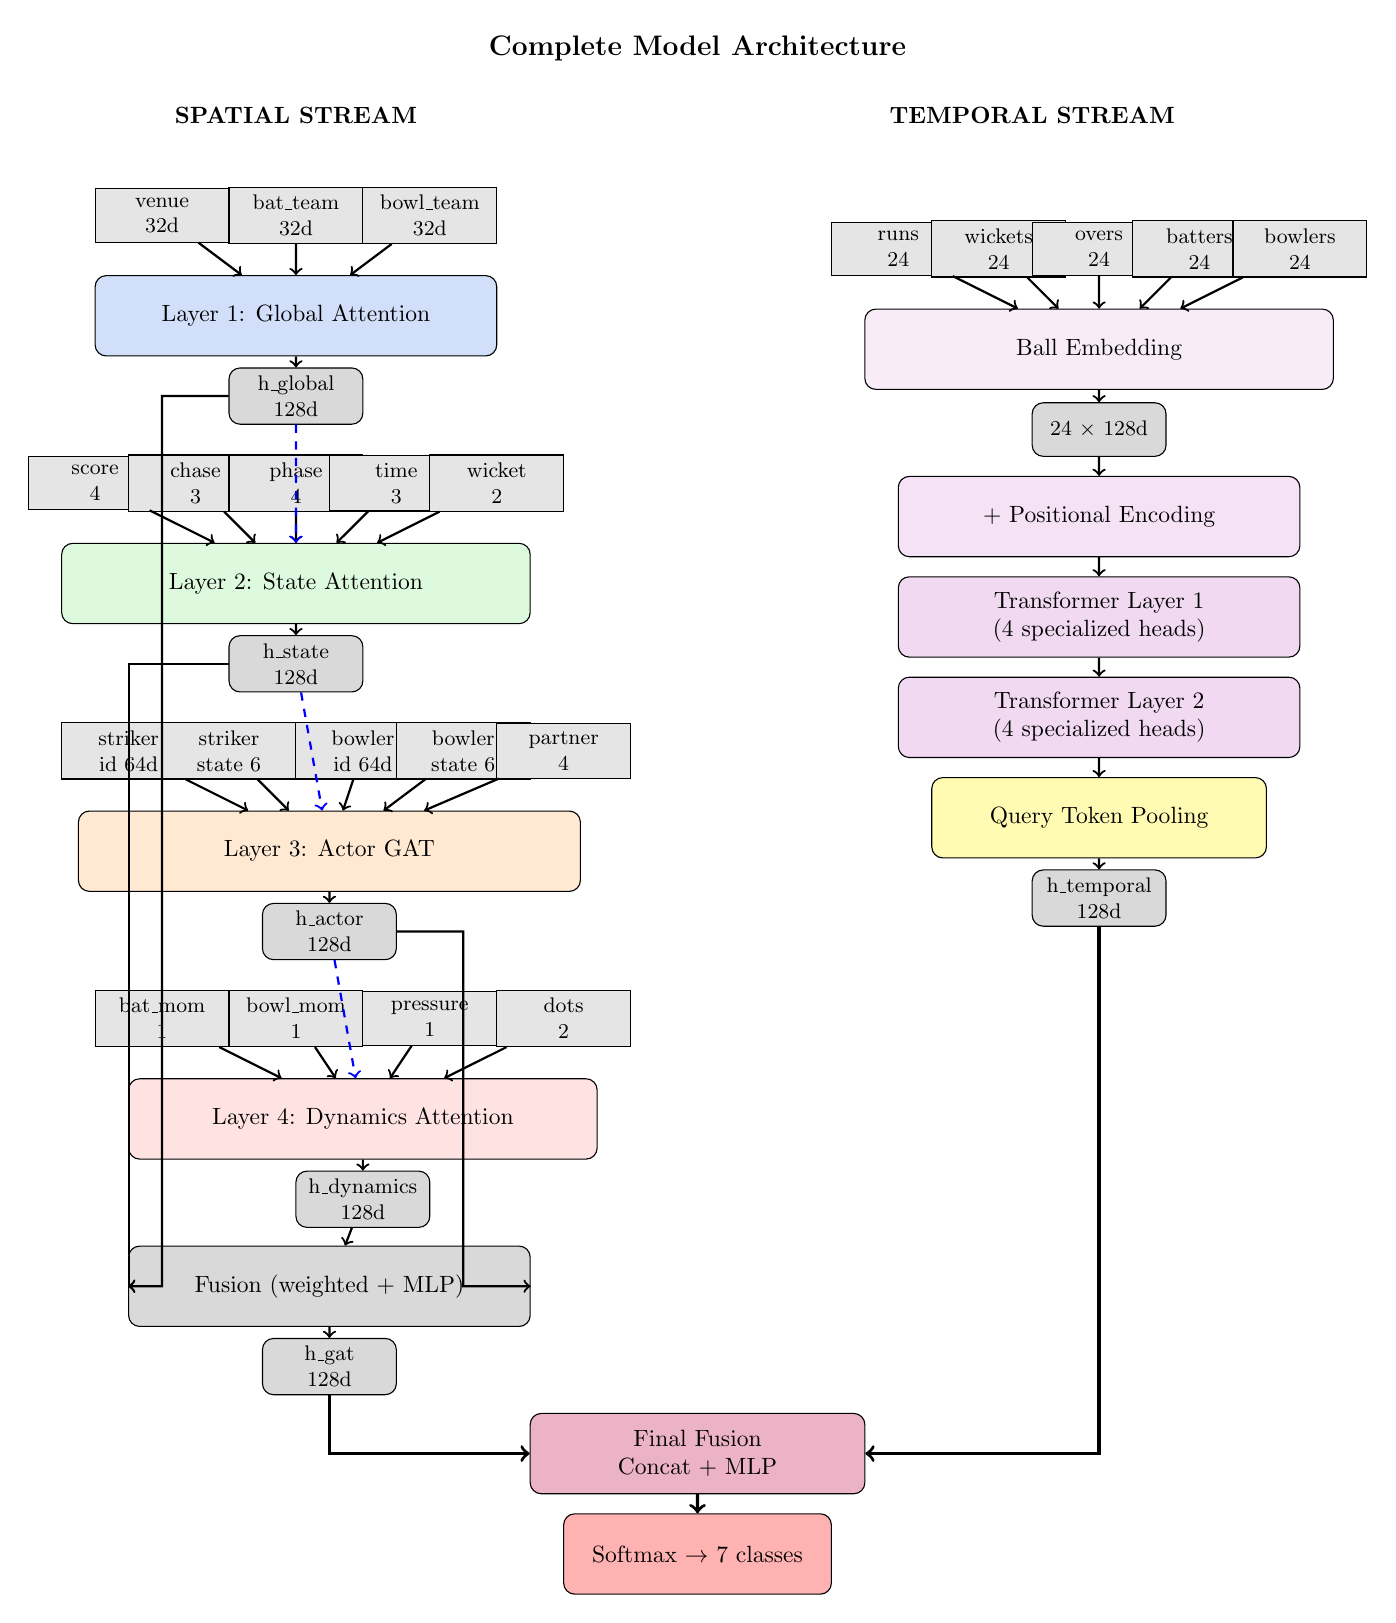
\begin{tikzpicture}[
    scale=0.85,
    transform shape,
    input/.style={rectangle, draw, fill=gray!20, minimum width=2cm, minimum height=0.8cm, align=center, font=\small},
    layer/.style={rectangle, draw, rounded corners, minimum width=8cm, minimum height=1.2cm, align=center},
    output/.style={rectangle, draw, rounded corners, fill=gray!30, minimum width=2cm, minimum height=0.8cm, align=center, font=\small},
]
    % Title
    \node[font=\large\bfseries] at (0, 8) {Complete Model Architecture};

    % === SPATIAL STREAM (left) ===
    \node[font=\bfseries] at (-6, 7) {SPATIAL STREAM};

    % Layer 1
    \node[input] (v) at (-8, 5.5) {venue\\32d};
    \node[input] (bt) at (-6, 5.5) {bat\_team\\32d};
    \node[input] (bwt) at (-4, 5.5) {bowl\_team\\32d};
    \node[layer, fill=globalcolor!30, minimum width=6cm] (l1) at (-6, 4) {Layer 1: Global Attention};
    \node[output] (hg) at (-6, 2.8) {h\_global\\128d};

    \draw[->, thick] (v) -- (l1);
    \draw[->, thick] (bt) -- (l1);
    \draw[->, thick] (bwt) -- (l1);
    \draw[->, thick] (l1) -- (hg);

    % Layer 2
    \node[input] (sc) at (-9, 1.5) {score\\4};
    \node[input] (ch) at (-7.5, 1.5) {chase\\3};
    \node[input] (ph) at (-6, 1.5) {phase\\4};
    \node[input] (tm) at (-4.5, 1.5) {time\\3};
    \node[input] (wk) at (-3, 1.5) {wicket\\2};
    \node[layer, fill=statecolor!30, minimum width=7cm] (l2) at (-6, 0) {Layer 2: State Attention};
    \node[output] (hs) at (-6, -1.2) {h\_state\\128d};

    \foreach \n in {sc, ch, ph, tm, wk} {
        \draw[->, thick] (\n) -- (l2);
    }
    \draw[->, thick, dashed, blue] (hg) -- (l2);
    \draw[->, thick] (l2) -- (hs);

    % Layer 3
    \node[input] (si) at (-8.5, -2.5) {striker\\id 64d};
    \node[input] (ss) at (-7, -2.5) {striker\\state 6};
    \node[input] (bi) at (-5, -2.5) {bowler\\id 64d};
    \node[input] (bs) at (-3.5, -2.5) {bowler\\state 6};
    \node[input] (pt) at (-2, -2.5) {partner\\4};
    \node[layer, fill=actorcolor!30, minimum width=7.5cm] (l3) at (-5.5, -4) {Layer 3: Actor GAT};
    \node[output] (ha) at (-5.5, -5.2) {h\_actor\\128d};

    \foreach \n in {si, ss, bi, bs, pt} {
        \draw[->, thick] (\n) -- (l3);
    }
    \draw[->, thick, dashed, blue] (hs) -- (l3);
    \draw[->, thick] (l3) -- (ha);

    % Layer 4
    \node[input] (bm) at (-8, -6.5) {bat\_mom\\1};
    \node[input] (blm) at (-6, -6.5) {bowl\_mom\\1};
    \node[input] (pr) at (-4, -6.5) {pressure\\1};
    \node[input] (dp) at (-2, -6.5) {dots\\2};
    \node[layer, fill=dynamicscolor!30, minimum width=7cm] (l4) at (-5, -8) {Layer 4: Dynamics Attention};
    \node[output] (hd) at (-5, -9.2) {h\_dynamics\\128d};

    \foreach \n in {bm, blm, pr, dp} {
        \draw[->, thick] (\n) -- (l4);
    }
    \draw[->, thick, dashed, blue] (ha) -- (l4);
    \draw[->, thick] (l4) -- (hd);

    % Fusion
    \node[layer, fill=gray!30, minimum width=6cm] (fuse) at (-5.5, -10.5) {Fusion (weighted + MLP)};
    \node[output] (hgat) at (-5.5, -11.7) {h\_gat\\128d};

    \draw[->, thick] (hg) -- ++(-2,0) |- (fuse);
    \draw[->, thick] (hs) -- ++(-2.5,0) |- (fuse);
    \draw[->, thick] (ha) -- ++(2,0) |- (fuse);
    \draw[->, thick] (hd) -- (fuse);
    \draw[->, thick] (fuse) -- (hgat);

    % === TEMPORAL STREAM (right) ===
    \node[font=\bfseries] at (5, 7) {TEMPORAL STREAM};

    % Inputs
    \node[input] (runs) at (3, 5) {runs\\24};
    \node[input] (wkts) at (4.5, 5) {wickets\\24};
    \node[input] (ovrs) at (6, 5) {overs\\24};
    \node[input] (btrs) at (7.5, 5) {batters\\24};
    \node[input] (bwlrs) at (9, 5) {bowlers\\24};

    % Ball embed
    \node[layer, fill=temporalcolor!20, minimum width=7cm] (be) at (6, 3.5) {Ball Embedding};
    \node[output] (balls) at (6, 2.3) {24 $\times$ 128d};

    \foreach \n in {runs, wkts, ovrs, btrs, bwlrs} {
        \draw[->, thick] (\n) -- (be);
    }
    \draw[->, thick] (be) -- (balls);

    % Pos encoding
    \node[layer, fill=temporalcolor!30, minimum width=6cm] (pe) at (6, 1) {+ Positional Encoding};
    \draw[->, thick] (balls) -- (pe);

    % Transformer layers
    \node[layer, fill=temporalcolor!40, minimum width=6cm] (tf1) at (6, -0.5) {Transformer Layer 1\\(4 specialized heads)};
    \node[layer, fill=temporalcolor!40, minimum width=6cm] (tf2) at (6, -2) {Transformer Layer 2\\(4 specialized heads)};

    \draw[->, thick] (pe) -- (tf1);
    \draw[->, thick] (tf1) -- (tf2);

    % Query pooling
    \node[layer, fill=yellow!30, minimum width=5cm] (qp) at (6, -3.5) {Query Token Pooling};
    \node[output] (ht) at (6, -4.7) {h\_temporal\\128d};

    \draw[->, thick] (tf2) -- (qp);
    \draw[->, thick] (qp) -- (ht);

    % === FINAL FUSION ===
    \node[layer, fill=purple!30, minimum width=5cm] (final) at (0, -13) {Final Fusion\\Concat + MLP};
    \node[layer, fill=red!30, minimum width=4cm] (pred) at (0, -14.5) {Softmax $\to$ 7 classes};

    \draw[->, very thick] (hgat) |- (final);
    \draw[->, very thick] (ht) |- (final);
    \draw[->, very thick] (final) -- (pred);

\end{tikzpicture}
\caption{Complete architecture with all inputs, layers, and outputs}
\end{figure}

%==========================================
\newpage
\section{Feature Reference Tables}
%==========================================

\subsection{All 17 Spatial Nodes}

\begin{table}[H]
\centering
\small
\begin{tabular}{llcll}
\toprule
Layer & Node Name & Input Dim & Features & Intuition \\
\midrule
\multirow{3}{*}{Global}
    & venue & 32 & Learned embedding & Ground characteristics \\
    & batting\_team & 32 & Learned embedding & Team's batting DNA \\
    & bowling\_team & 32 & Learned embedding & Team's bowling style \\
\midrule
\multirow{5}{*}{State}
    & score\_state & 4 & score, wickets, balls, innings & Current score \\
    & chase\_state & 3 & runs\_needed, RRR, is\_chase & Chase equation \\
    & phase\_state & 4 & powerplay, middle, death, progress & Match phase \\
    & time\_pressure & 3 & balls\_left, urgency, is\_death & Time remaining \\
    & wicket\_buffer & 2 & wickets\_in\_hand, is\_danger & Wicket cushion \\
\midrule
\multirow{5}{*}{Actor}
    & striker\_identity & 64 & Learned embedding & WHO is batting \\
    & striker\_state & 6 & runs, balls, SR, dots, set, bdry & HOW batter is doing \\
    & bowler\_identity & 64 & Learned embedding & WHO is bowling \\
    & bowler\_state & 6 & balls, runs, wkts, econ, dots, threat & HOW bowler is doing \\
    & partnership & 4 & runs, balls, RR, stability & Partnership health \\
\midrule
\multirow{4}{*}{Dynamics}
    & batting\_momentum & 1 & recent\_RR vs expected & Scoring momentum \\
    & bowling\_momentum & 1 & inverse of batting & Bowling control \\
    & pressure\_index & 1 & composite pressure & Overall pressure \\
    & dot\_pressure & 2 & consec\_dots, since\_boundary & Building pressure \\
\bottomrule
\end{tabular}
\caption{Complete feature reference for all 17 spatial nodes}
\end{table}

\subsection{Temporal Features (per ball)}

\begin{table}[H]
\centering
\begin{tabular}{lcl}
\toprule
Feature & Dimension & Description \\
\midrule
runs & 1 & Runs scored on this ball (normalized) \\
wicket & 1 & 1 if wicket fell, 0 otherwise \\
over\_progress & 1 & Which over this ball was in (normalized) \\
batter\_id & 32 & Embedding of batter who faced this ball \\
bowler\_id & 32 & Embedding of bowler who bowled this ball \\
\midrule
\textbf{Total per ball} & \textbf{128} & After projection and concatenation \\
\textbf{Sequence length} & \textbf{24} & Last 4 overs of history \\
\bottomrule
\end{tabular}
\caption{Temporal input features}
\end{table}

%==========================================
\section{Key Design Decisions}
%==========================================

\begin{table}[H]
\centering
\begin{tabular}{p{4cm}p{5cm}p{5cm}}
\toprule
Decision & Current Choice & Alternative \\
\midrule
Spatial vs Temporal & Parallel streams & Sequential (GAT per ball, then temporal attention) \\
\addlinespace
Actor layer & GATv2 with fixed edges & Full attention or learned edges \\
\addlinespace
Temporal heads & 3 specialized + 1 free & All learned or all specialized \\
\addlinespace
History length & 24 balls (4 overs) & Full innings (more expensive) \\
\addlinespace
Layer fusion & Weighted sum + concat & Only weighted or only concat \\
\addlinespace
Graph structure & Treated as homogeneous & PyG heterogeneous graph \\
\bottomrule
\end{tabular}
\caption{Key architectural decisions and alternatives}
\end{table}

\section{What Each Output Represents}

\begin{table}[H]
\centering
\begin{tabular}{lp{10cm}}
\toprule
Output & Intuitive Meaning \\
\midrule
h\_global & ``The setting'' --- venue + team context compressed into one vector \\
h\_state & ``The situation'' --- current match state (score, phase, pressure) \\
h\_actor & ``The protagonists'' --- who's batting, who's bowling, their duel \\
h\_dynamics & ``The pulse'' --- current momentum and pressure \\
h\_gat & Complete spatial understanding of this moment \\
h\_temporal & Patterns from recent history (last 4 overs) \\
\textbf{Final output} & 7 probabilities: dot, 1, 2, 3, 4, 6, wicket \\
\bottomrule
\end{tabular}
\caption{Intuitive interpretation of each intermediate output}
\end{table}

\end{document}
